
The resulting fits to the inclusive m$(4\ell)$ distributions for the integrated $\Hllll$ fiducial cross section measurements for different final states, 
performed in the $m_{4\ell}$ range from 105~GeV to 140~GeV, are shown in Figure~\ref{fig:sigfits-data-SM-inclusive}. The extracted inclusive cross sections as function of center of mass energy are shown in Figure~\ref{fig:inclusive-results:a} while the extracted integrated cross section results for different final states at 13~TeV corresponding to different data taking periods are shown in Figure~\ref{fig:inclusive-results:b}. 
The red error bar represents the systematic uncertainty, while black error bar represents the combined statistical and 
systematic uncertainties, summed in quadrature. The sub-dominant component of the signal XH $=$ VBF $+$ VH $+$ $\ttH$ is indicated in green separately. 
%The additional systematic uncertainty associated with the model dependence
%is separately represented by a grey box. 
Above listed results are summarized in Tables \ref{tab:incresults} and \ref{tab:incresultsPAS}.
% Summary of individual measurements of inclusive $\Hllll$ fiducial cross sections at 7~TeV and 8~TeV, performed in the $m_{4\ell}$ range from 105~GeV 
% to 140~GeV,  are presented in Table~\ref{tab:incresults} and Figure~\ref{fig:inclusive-results-summary} and Figure~\ref{fig:ratio7o8-results-summary}.

The $\Hllll$ measurements are compared to the SM NNLO theoretical estimations where the acceptance of the 
dominant $\ggH$ contribution is modelled using {\sc powheg} at  $\sqrt{s}$=13\TeV and {\sc HRes}~\cite{Grazzini:2013mca,deFlorian:2012mx} at  $\sqrt{s}$=7 and 8\TeV and the total gluon fusion cross section and uncertainty  
are taken from Ref.~\cite{Anastasiou2016}. The fiducial volume for $\sqrt{s}$=6--9\TeV uses the lepp
ton isolation definition from Ref.~\cite{CMSH4lFiducial8TeV}, while for $\sqrt{s}$=12--14\TeV the definition descrr
ibed in the text is used.

%Total uncertainty on NNLL+NNLO theoretical computations is obtained from Ref.~\cite{LHCHiggsCrossSectionWorkingGroup:2013tqa} and includes
%uncertainties due to the renormalization and factorization scales ($\sim 7.8\%$), PDFs ($\sim 7.5\%$),branching fraction (2\%) and acceptance ($2\%$). For
%total theoretical uncertainty calculations, PDFs/$\alpha_{\rm S}$ uncertainties are considered to be corrected between VH and VBF production mechanism
%(dominantly quark-antiquark initiated) and anti-correlated between $\ttH$ and $\ggH$ mechanism (dominantly gluon-gluon initiated). Furthermore, uncertainties
%due to DCQ scale are assumed to be uncorrelated, while acceptance and branching fraction uncertainties are assumed to be corrected among all production mechanism.
%In all figures, the theoretical estimations that used {\sc HRes}, {\sc powheg+JHUgen} and {\sc powheg minlo-HJ}
% for the description of the gg$\rightarrow$H process are shown in pink, blue and yellow, respectively, while the sub-dominant component of the 
% signal XH $=$ VBF $+$ VH $+$ $\ttH$ is indicated in green separately.
%A small difference between the predictions based on {\sc powheg+JHUgen} and {\sc minloHJ}
% is arising from the way the acceptance of the gg$\rightarrow$H contribution is modelled by these two generators.
When extracting the total H$\rightarrow4\ell$ fiducial cross section, the parameter of interest is the total fiducial cross section and the fractions of $4e,4\mu,$ and $2e2\mu$ is floated in the fit. When extracting the fiducial cross section for each final state, the three parameters of interest are the cross sections of three individual final states.

\begin{figure}[!htb]
  \begin{center}
    \subfigure[$4e$]{
      %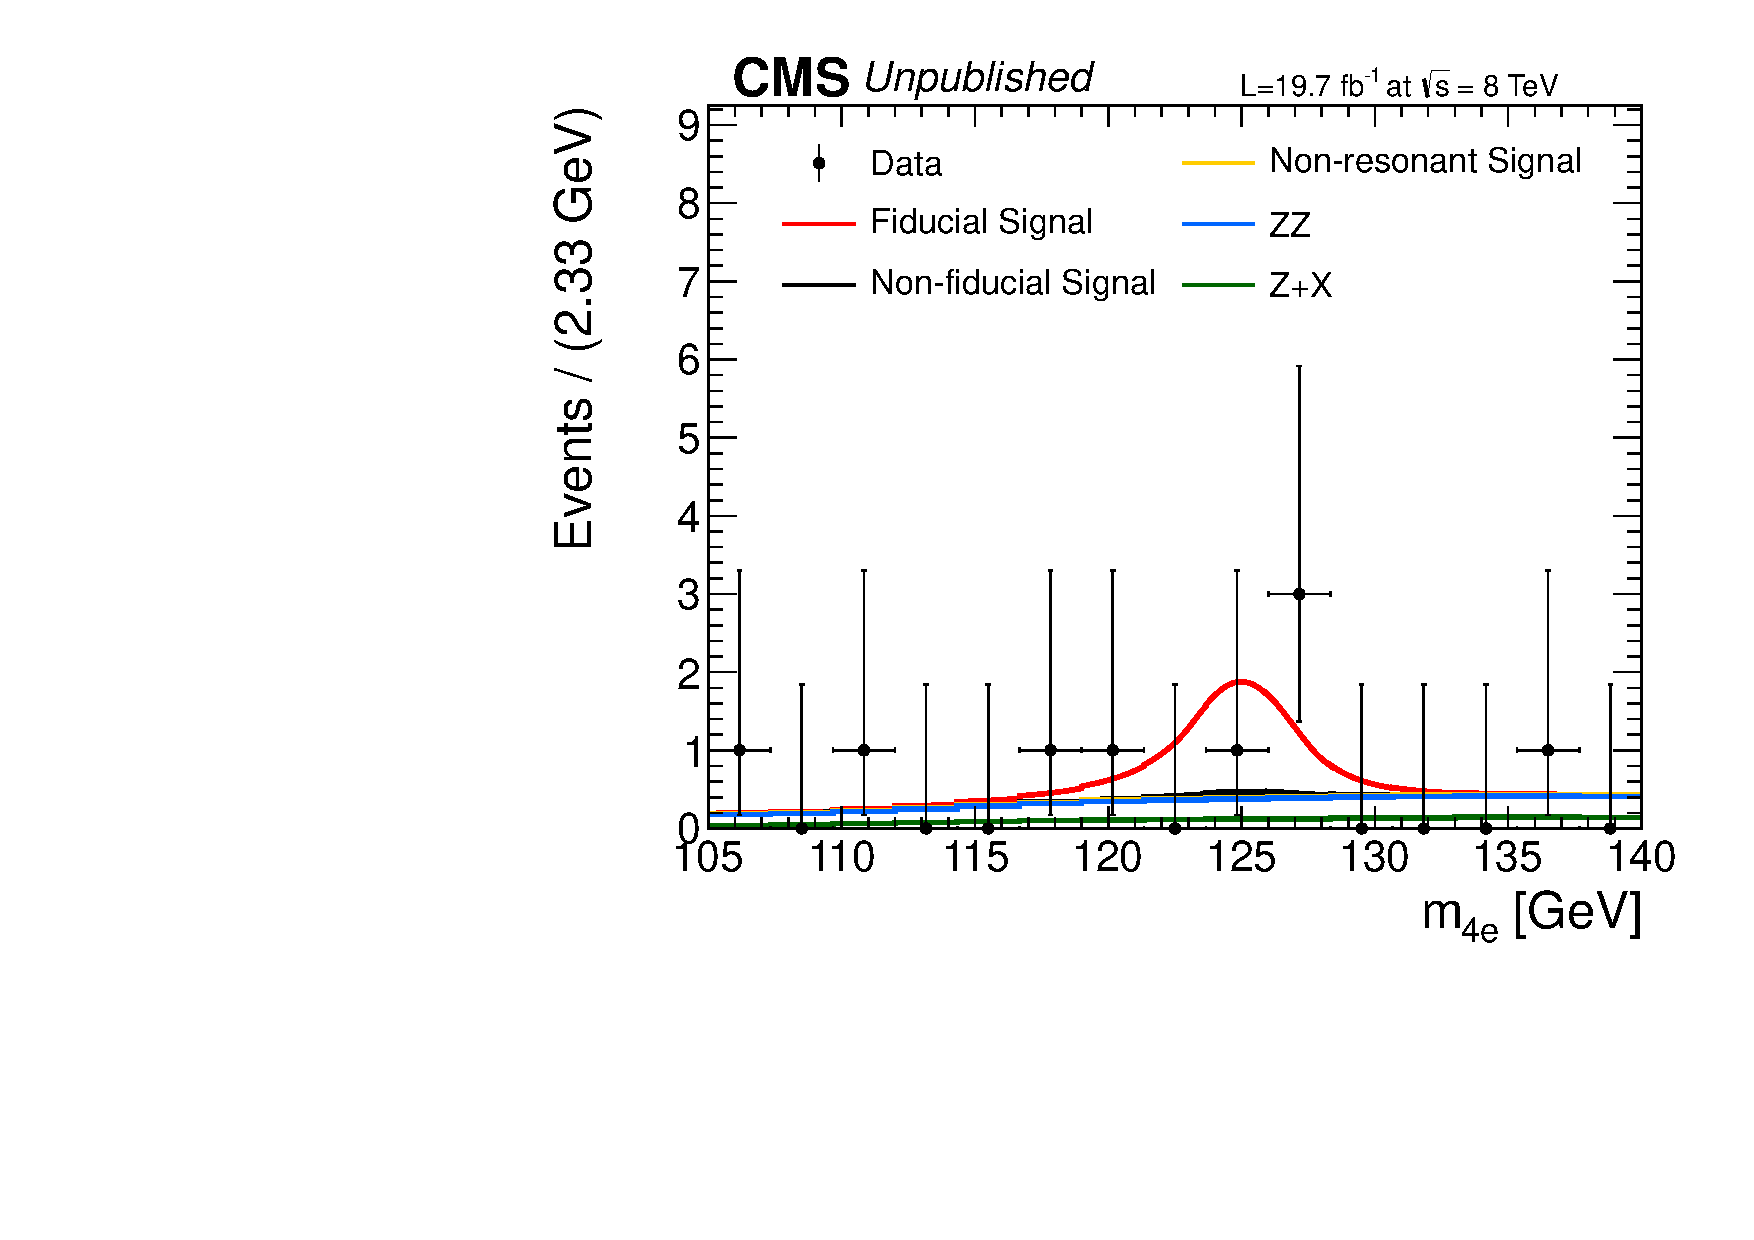
\includegraphics[width=0.48\textwidth,angle=0]{Plots/data_unfoldwith_SM_125_v2_mass4l_4e_recobin0_unpublished.pdf}
      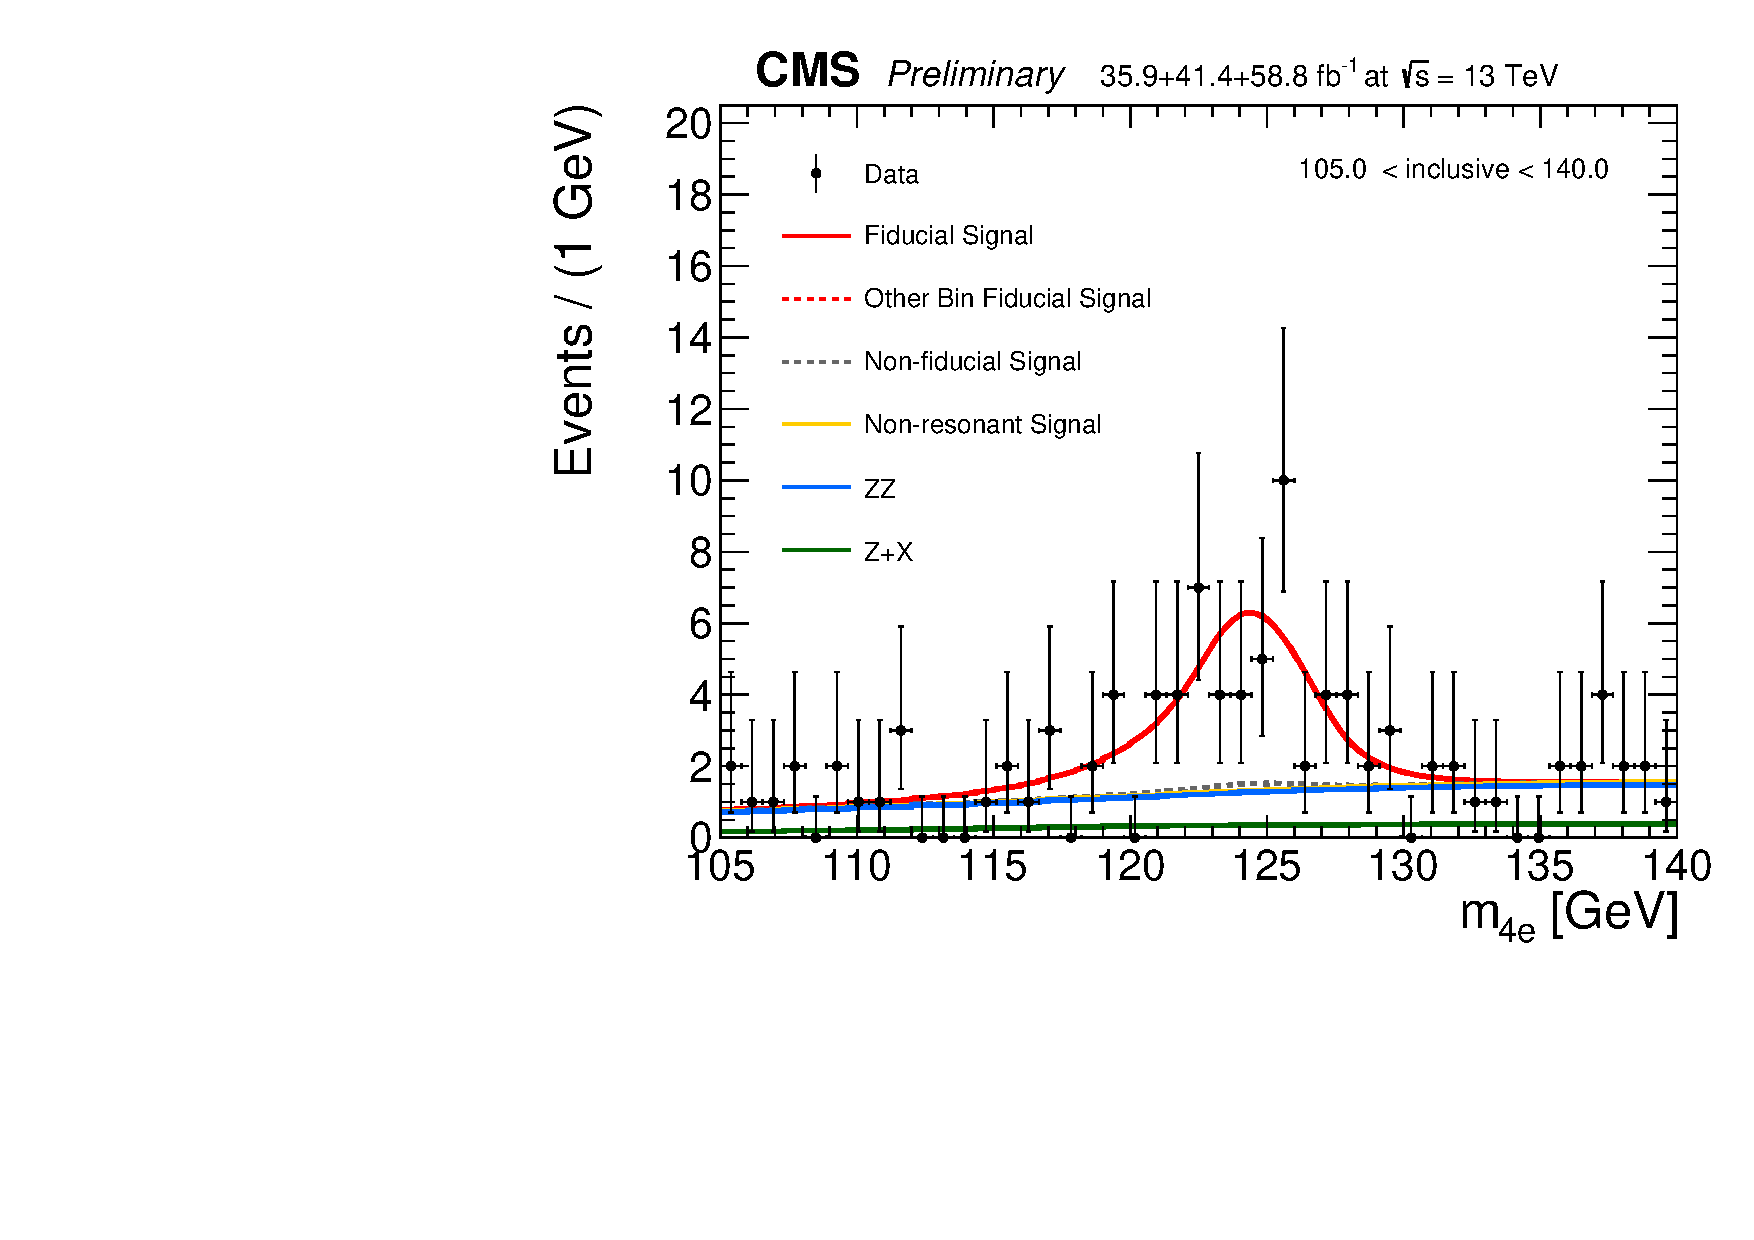
\includegraphics[width=0.48\textwidth,angle=0]{Plots/data_unfoldwith_SM_125_v3_mass4l_4e_recobin0.pdf}
       \label{fig:sigfits-data-SM-inclusive:a}
    }
    \subfigure[$4\mu$]{
      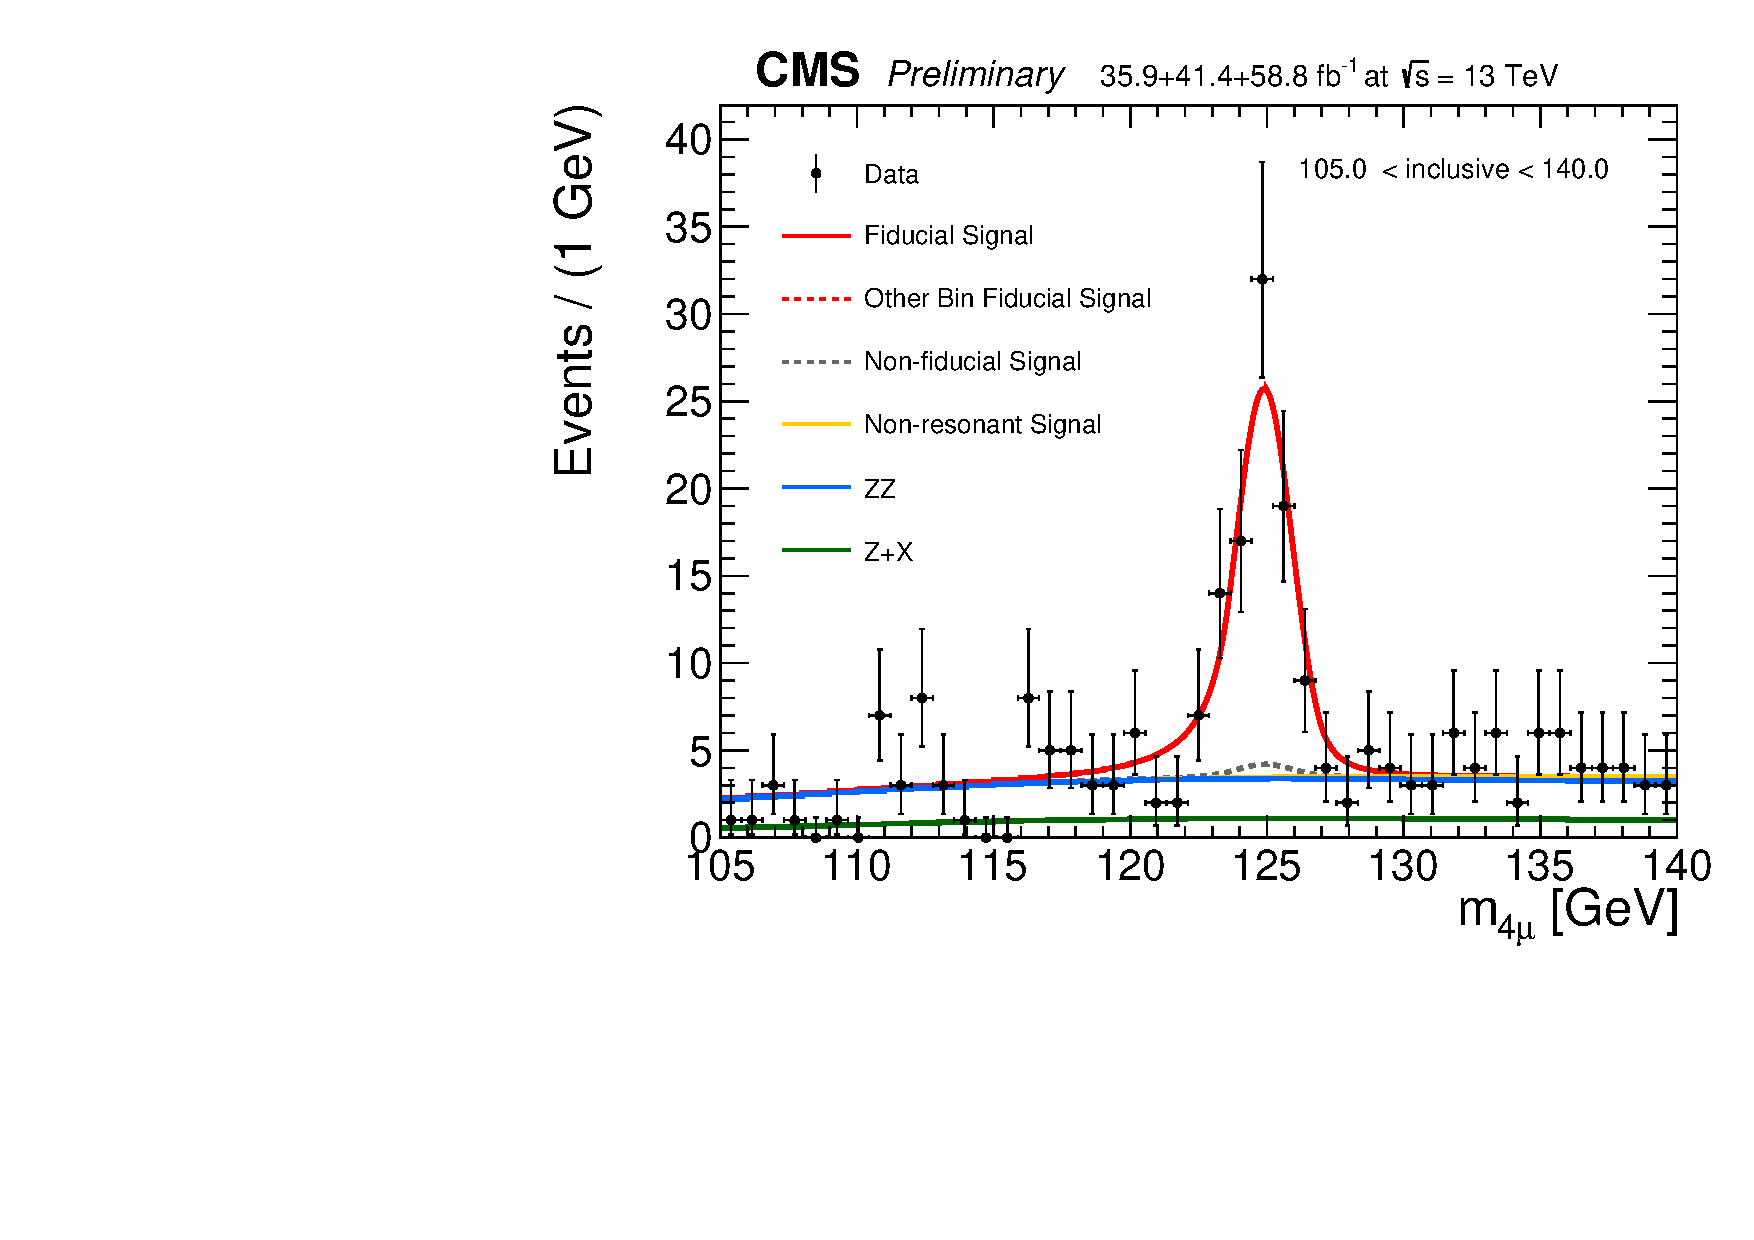
\includegraphics[width=0.48\textwidth,angle=0]{Plots/data_unfoldwith_SM_125_v3_mass4l_4mu_recobin0.pdf}
       \label{fig:sigfits-data-SM-inclusive:b}
    } \\
    \subfigure[$2e2\mu$]{
      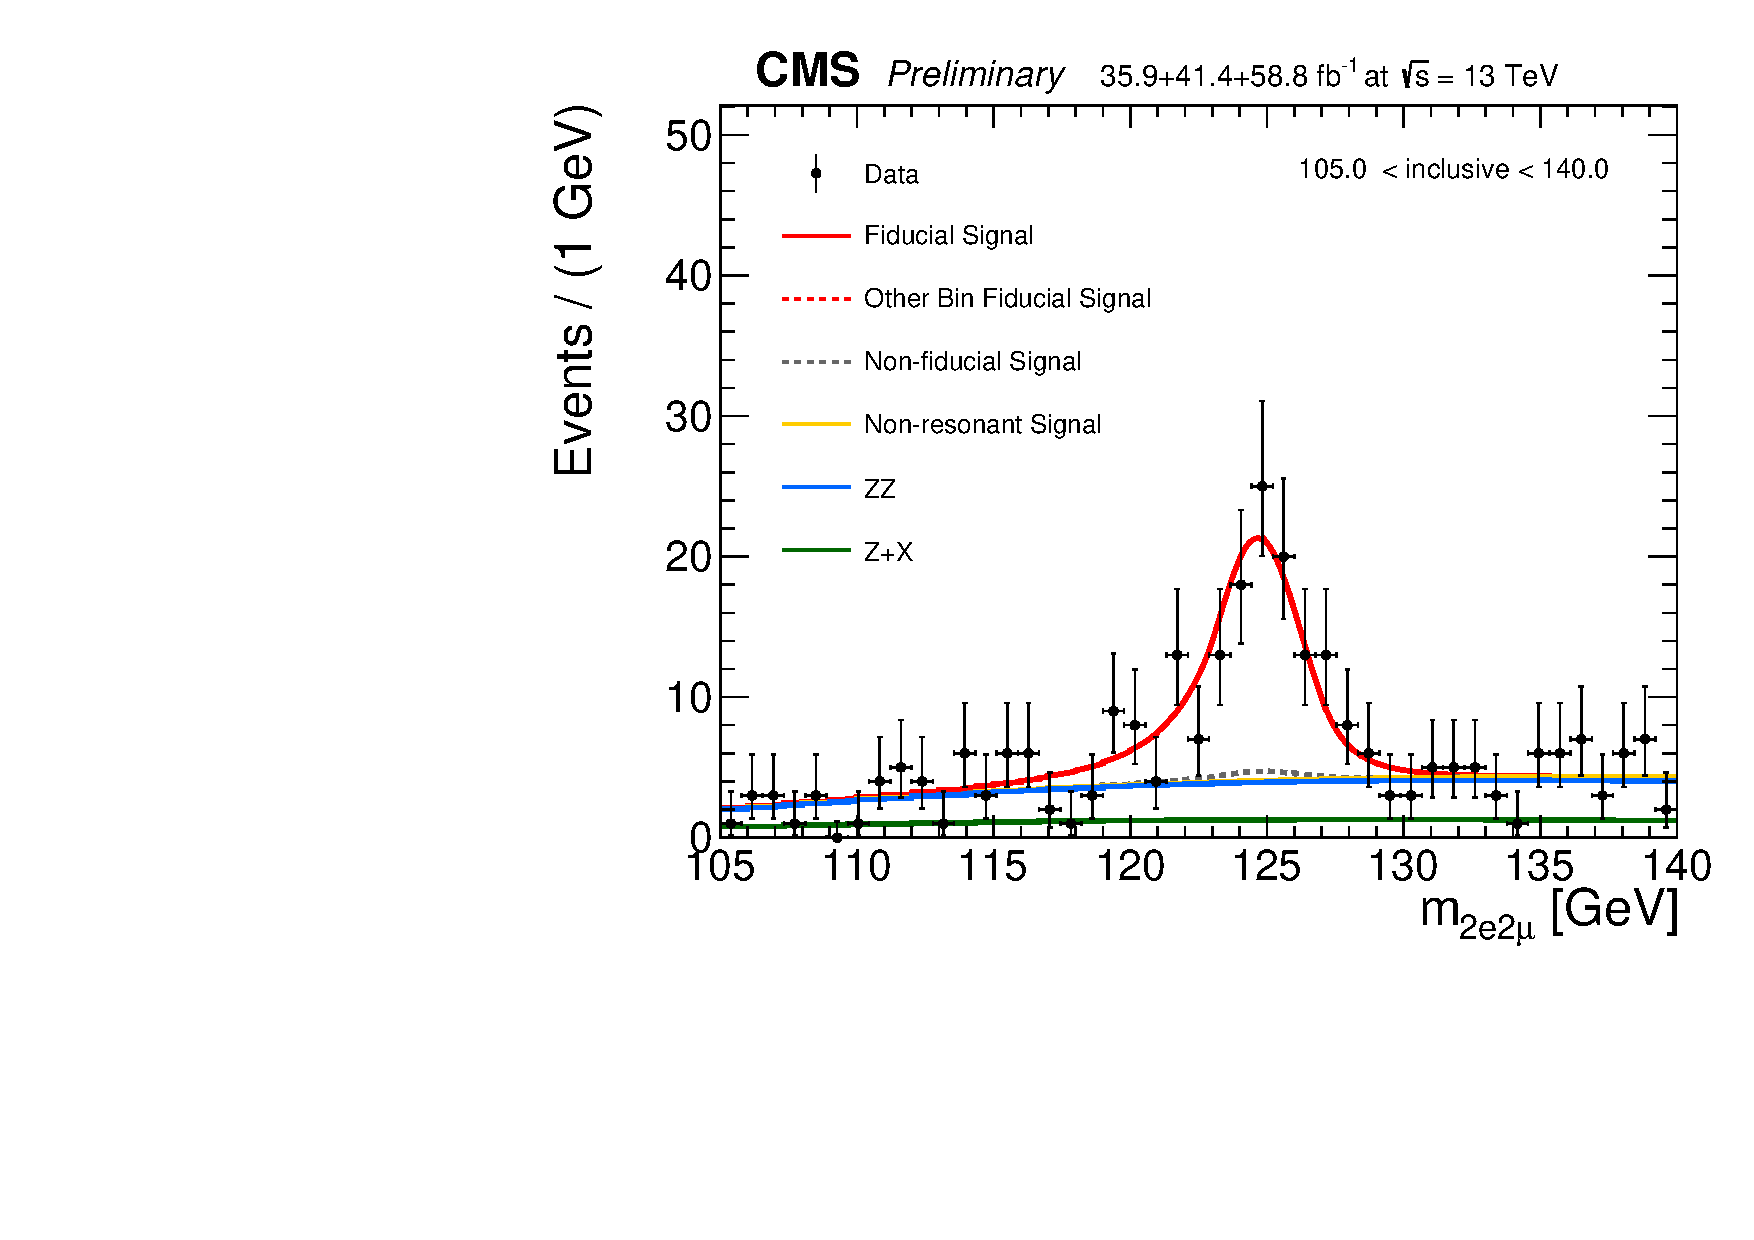
\includegraphics[width=0.48\textwidth,angle=0]{Plots/data_unfoldwith_SM_125_v3_mass4l_2e2mu_recobin0.pdf}
       \label{fig:sigfits-data-SM-inclusive:c}
    }
    \subfigure[$4\ell$]{
      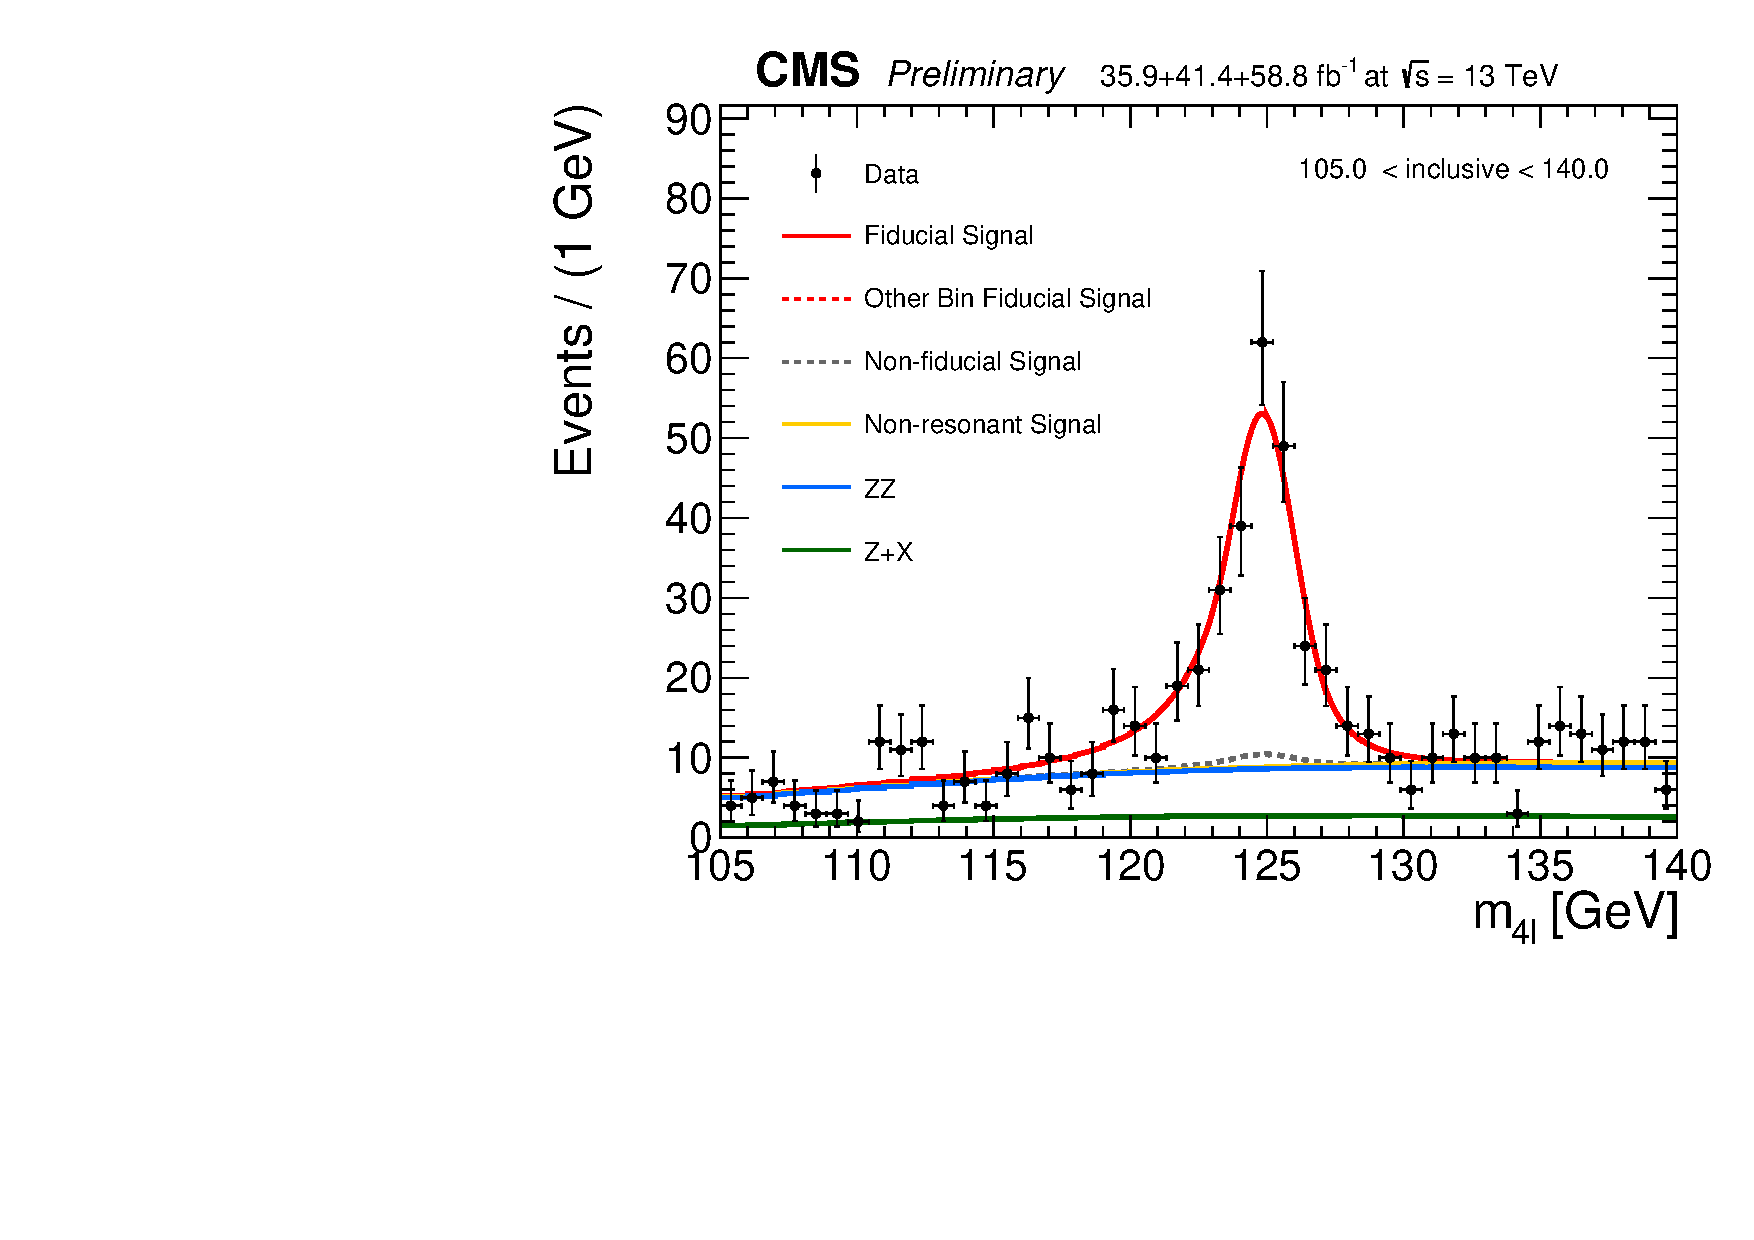
\includegraphics[width=0.48\textwidth,angle=0]{Plots/data_unfoldwith_SM_125_v3_mass4l_4l_recobin0.pdf}
       \label{fig:sigfits-data-SM-inclusive:d}
    } \\
    \caption{Inclusive four lepton mass distributions in data and the resulting fitted values of the signal and background pdfs in different final states.}
  \label{fig:sigfits-data-SM-inclusive}
  \end{center}
\end{figure}
%%%%%%%%
\begin{figure}[!htb]
  \begin{center}  
    \subfigure[$\Hllll$ (7, 8 and 13 TeV)]{
      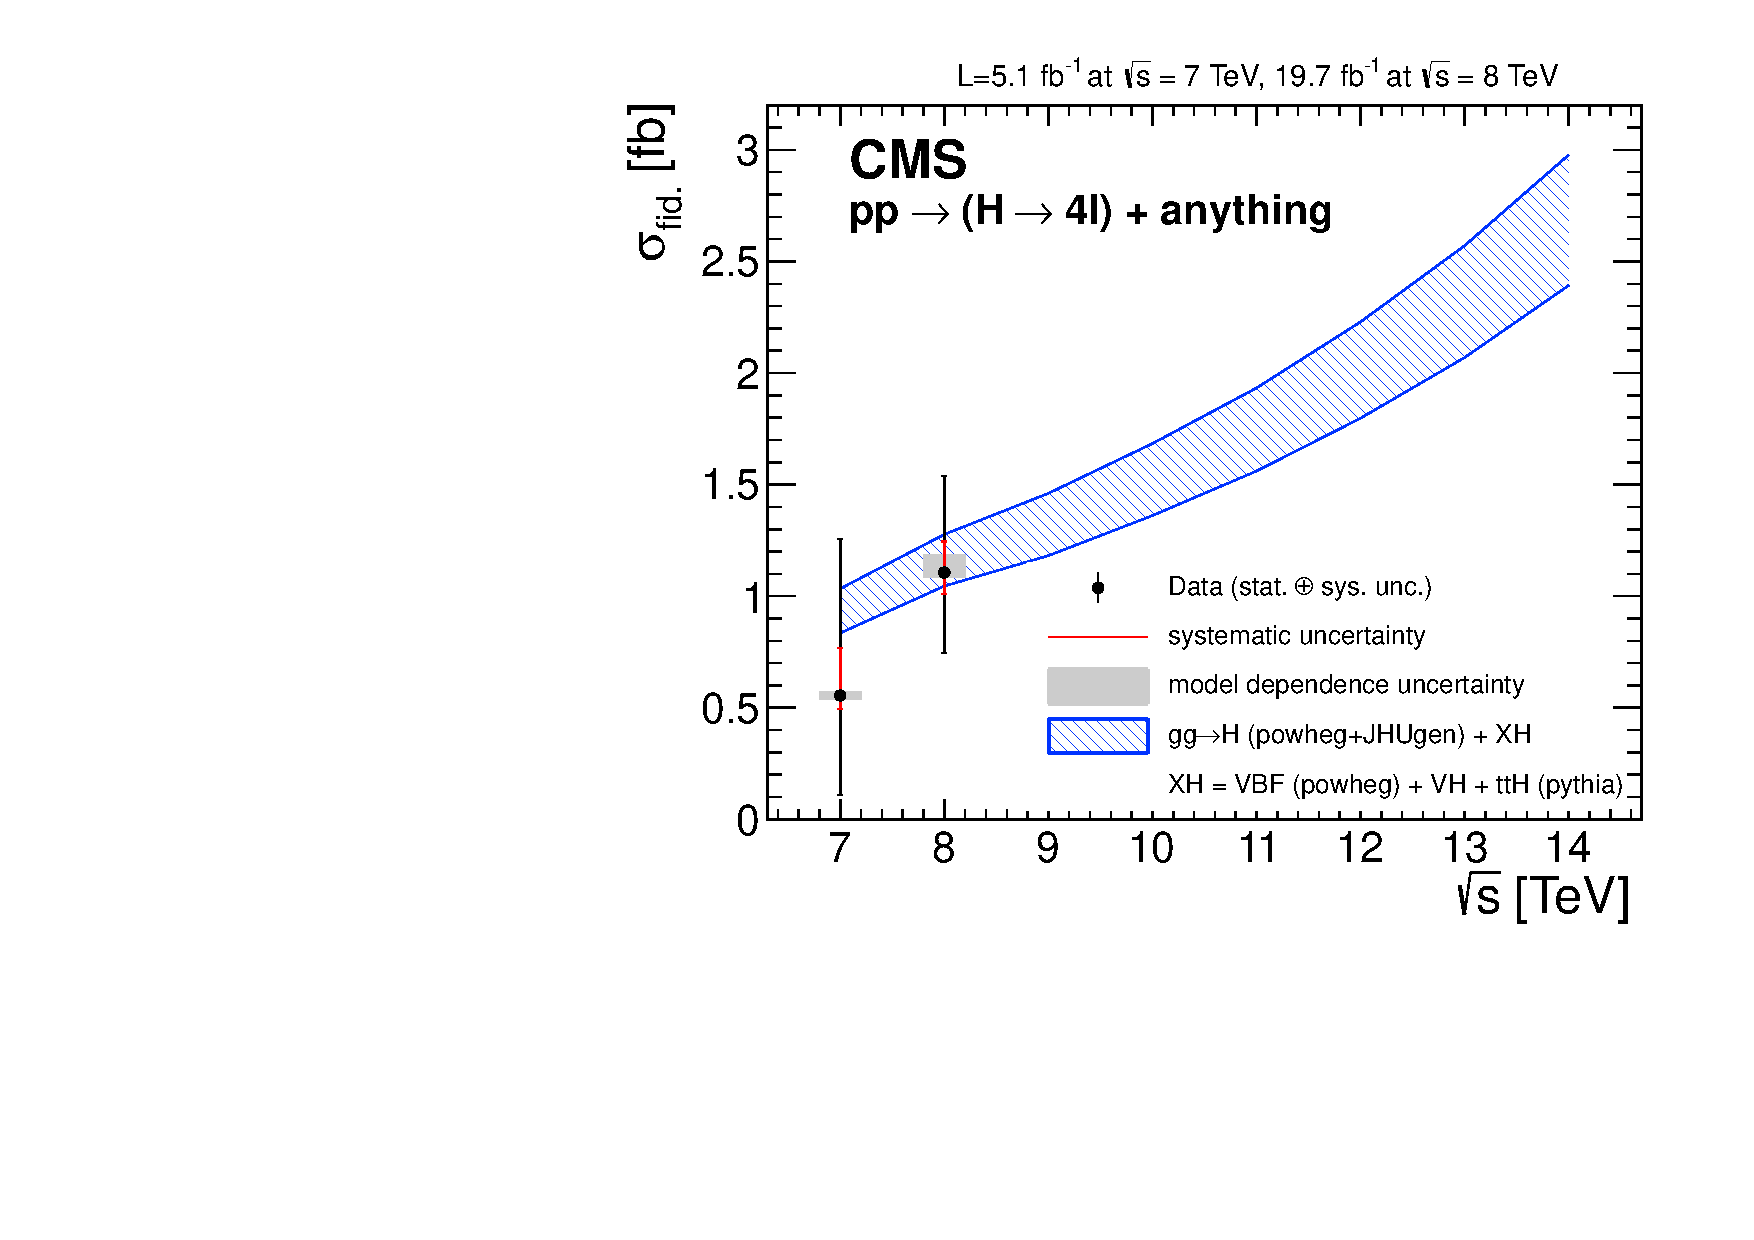
\includegraphics[width=0.48\textwidth,angle=0]{Plots/xs_vs_sqrts.pdf}
      \label{fig:inclusive-results:a}
    }
    \subfigure[$\Hllll$ (13 TeV)]{
      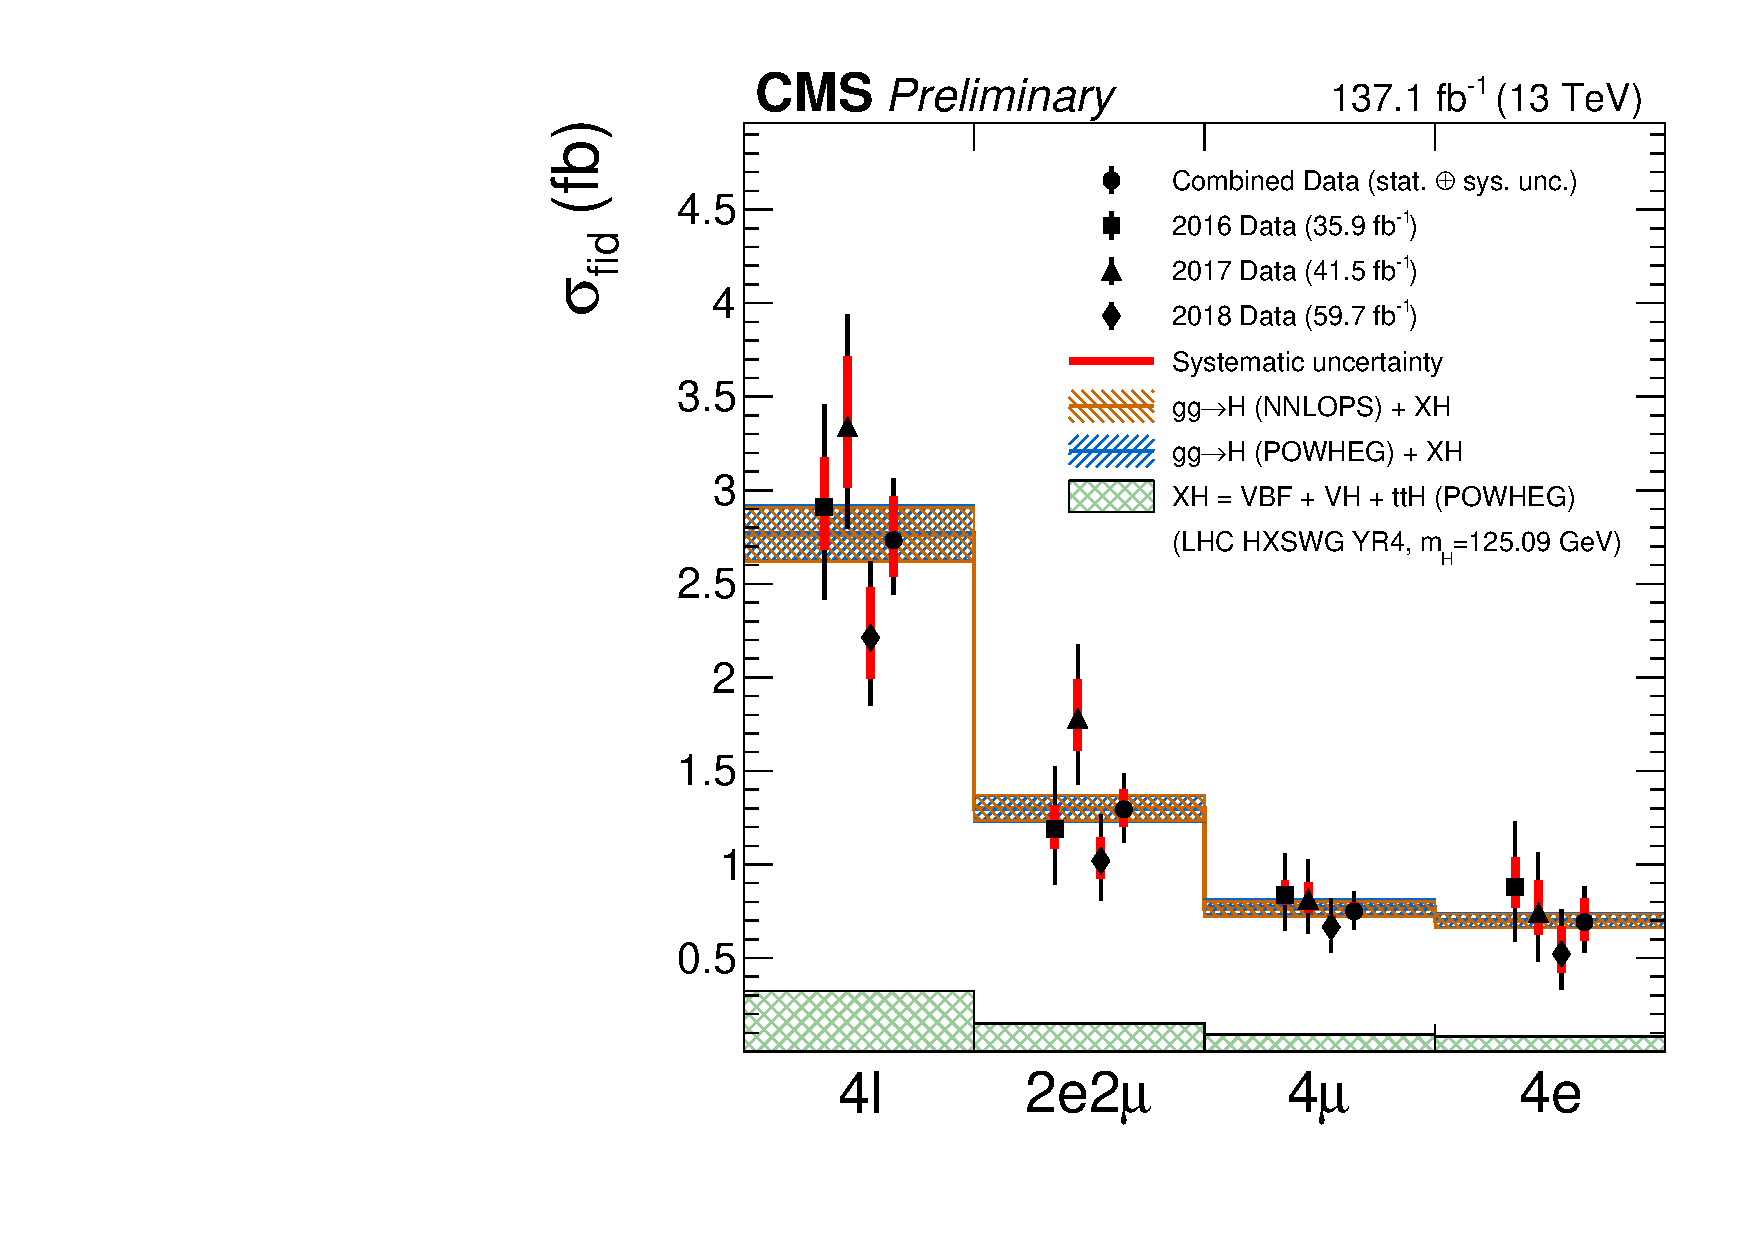
\includegraphics[width=0.48\textwidth,angle=0]{Plots/mass4l_unfoldwith_SM_125_ThreeYears.pdf}
      \label{fig:inclusive-results:b}
    }
 
    \caption{The measured fiducial cross section as a function of $\sqrt{s}$ (left). The measured inclusive fiducial cross section in different final states (right). % add refs. from AN-18-340  
                The acceptance is calculated using \POWHEG at  $\sqrt{s}$=13\TeV and {\sc HRes}~\cite{Grazzini:2013mca,deFlorian:2012mx} 
                at  $\sqrt{s}$=7 and 8\TeV and the total gluon fusion cross section and uncertainty are taken from 
                Ref.~\cite{Anastasiou2016}. The fiducial volume for $\sqrt{s}$=6--9\TeV uses the lepton isolation definition from 
                Ref.~\cite{CMSH4lFiducial8TeV}, while for $\sqrt{s}$=12--14\TeV the definition described in the text is used.

    } 
  \label{fig:inclusive-results}
 \end{center}
\end{figure}


%============
\begin{table}[!h!tb]
\begin{center}
      \caption{
Results of the $\Hllll$ integrated fiducial cross section measurements performed in the $m_{4\ell}$ range from 105~GeV to 140~GeV for proton 
collisions at 13~TeV.
        } \label{tab:incresults}
\begin{tabular}{|c|c|}
\hline %---------------------------------------------------------
\hline %---------------------------------------------------------
\multicolumn{2}{|c|}{ \textbf{Fiducial cross section $\Hllll$ at 13~TeV}} \\
\hline %---------------------------------------------------------
\vspace{-0.4cm} & \\
%Measured & $0.94^{\rm +0.79}_{\rm -0.57} \, {\rm(stat.)}\, ^{\rm +0.22}_{\rm -0.18}\,  {\rm (sys.)} \, ^{+0.04}_{-0.03}\,  {\rm (model)}\, {\rm fb}$  \\
%Measured & $0.56^{\rm +0.67}_{\rm -0.44} \, {\rm(stat.)}\, ^{\rm +0.21}_{\rm -0.06}\,  {\rm (sys.)} \, ^{+0.02}_{-0.02}\,  {\rm (model)}\, {\rm fb}$  \\
Measured & $2.73^{+0.30}_{-0.29}=2.73^{+0.23}_{-0.22}({\rm stat.})^{+0.24}_{-0.19}({\rm syst.})~{\rm fb}$  {\rm (model)} \\
\vspace{-0.4cm} & \\
\hline %---------------------------------------------------------
\vspace{-0.4cm} & \\
%Measured & $0.94^{\rm +0.79}_{\rm -0.57} \, {\rm(stat.)}\, ^{\rm +0.22}_{\rm -0.18}\,  {\rm (sys.)} \, ^{+0.04}_{-0.03}\,  {\rm (model)}\, {\rm fb}$  \\
\small gg$\rightarrow$H({\sc powheg}) + XH & $0.93^{\rm +0.10}_{\rm -0.11}{\rm fb}$ \\
\vspace{-0.4cm} & \\
\hline %---------------------------------------------------------
\vspace{-0.4cm} & \\
\small gg$\rightarrow$H({\sc NNLOPS}) + XH & $0.94^{\rm +0.10}_{\rm -0.10}{\rm fb}$ \\ 
%\vspace{-0.4cm} & \\
\hline %---------------------------------------------------------
%\vspace{-0.4cm} & \\
%%\small gg$\rightarrow$H({\sc minloHJJ}) + XH & $0.92^{\rm +0.10}_{\rm -0.10} {\rm fb}$ \\ 
%\small gg$\rightarrow$H({\sc minloHJ}) + XH & $0.93^{\rm +0.10}_{\rm -0.10} {\rm fb}$ \\ 
%\hline %---------------------------------------------------------
%\hline %---------------------------------------------------------
%\multicolumn{2}{|c|}{\textbf{Fiducial cross section $\Hllll$ at 8~TeV}} \\
%\hline %---------------------------------------------------------
%\vspace{-0.4cm} & \\
%Measured & $1.11^{\rm +0.41}_{\rm -0.35} \, {\rm(stat.)}\, ^{\rm +0.14}_{\rm -0.10}\,  {\rm (sys.)} \, ^{+0.08}_{-0.02}\,  {\rm (model)}\, {\rm fb}$  \\
%\vspace{-0.4cm} & \\
%\hline %---------------------------------------------------------
%\vspace{-0.4cm} & \\
%\small $\ggH$({\sc hres}) + XH & $1.15^{+0.12}_{-0.13}~{\rm fb}$ \\
%\vspace{-0.4cm} & \\
%\hline %---------------------------------------------------------
%\vspace{-0.4cm} & \\
%\small $\ggH$({\sc powheg+JHUgen}) + XH & $1.16^{+0.11}_{-0.11}~{\rm fb}$ \\ 
%\vspace{-0.4cm} & \\
%\hline %---------------------------------------------------------
%\vspace{-0.4cm} & \\
%%\small $\ggH$({\sc minloHJJ}) + XH & $1.14^{+0.12}_{-0.12} {\rm fb}$ \\ 
%\small $\ggH$({\sc minloHJ}) + XH & $1.17^{+0.11}_{-0.11}~{\rm fb}$ \\ 
%\hline %---------------------------------------------------------
%\hline %---------------------------------------------------------
%\multicolumn{2}{|c|}{\textbf{Ratio of fiducial cross sections of H$\rightarrow 4l$ at 7 and 8~TeV}} \\
%\hline %---------------------------------------------------------
%\vspace{-0.4cm} & \\
%%Measured & $0.81^{\rm +0.84}_{\rm -0.51} \, {\rm(stat.)}\, ^{\rm +0.31}_{\rm -0.11}\,  {\rm (sys.)} \, ^{+0.00}_{-0.03}\,  {\rm (model)}\,$  \\
%Measured & $0.51^{\rm +0.71}_{\rm -0.40} \, {\rm(stat.)}\, ^{\rm +0.13}_{\rm -0.05}\,  {\rm (sys.)} \, ^{+0.00}_{-0.03}\,  {\rm (model)}\,$  \\
%\vspace{-0.4cm} & \\



%\hline %---------------------------------------------------------
%\small gg$\rightarrow$H({\sc HRes}) + XH & $0.805^{+0.003}_{-0.010}$ \\
%
%\hline %---------------------------------------------------------
%\vspace{-0.4cm} & \\
%\small gg$\rightarrow$H({\sc powheg+JHUgen}) + XH & $0.814^{\rm +0.000}_{\rm -0.001}$ \\
%%\small gg$\rightarrow$H({\sc powheg+JHUgen}) + XH & $0.81$ \\
%\hline %---------------------------------------------------------
%\vspace{-0.4cm} & \\
%\small gg$\rightarrow$H({\sc minloHJ}) + XH & $0.809^{\rm +0.000}_{\rm -0.001}$ \\
%%\small gg$\rightarrow$H({\sc minloHJ}) + XH & $0.81$ \\
%\hline %---------------------------------------------------------
\hline %---------------------------------------------------------
\end{tabular}
\end{center}
\end{table}
%==================
%\begin{figure}[!h!tb]
% \begin{center}
%    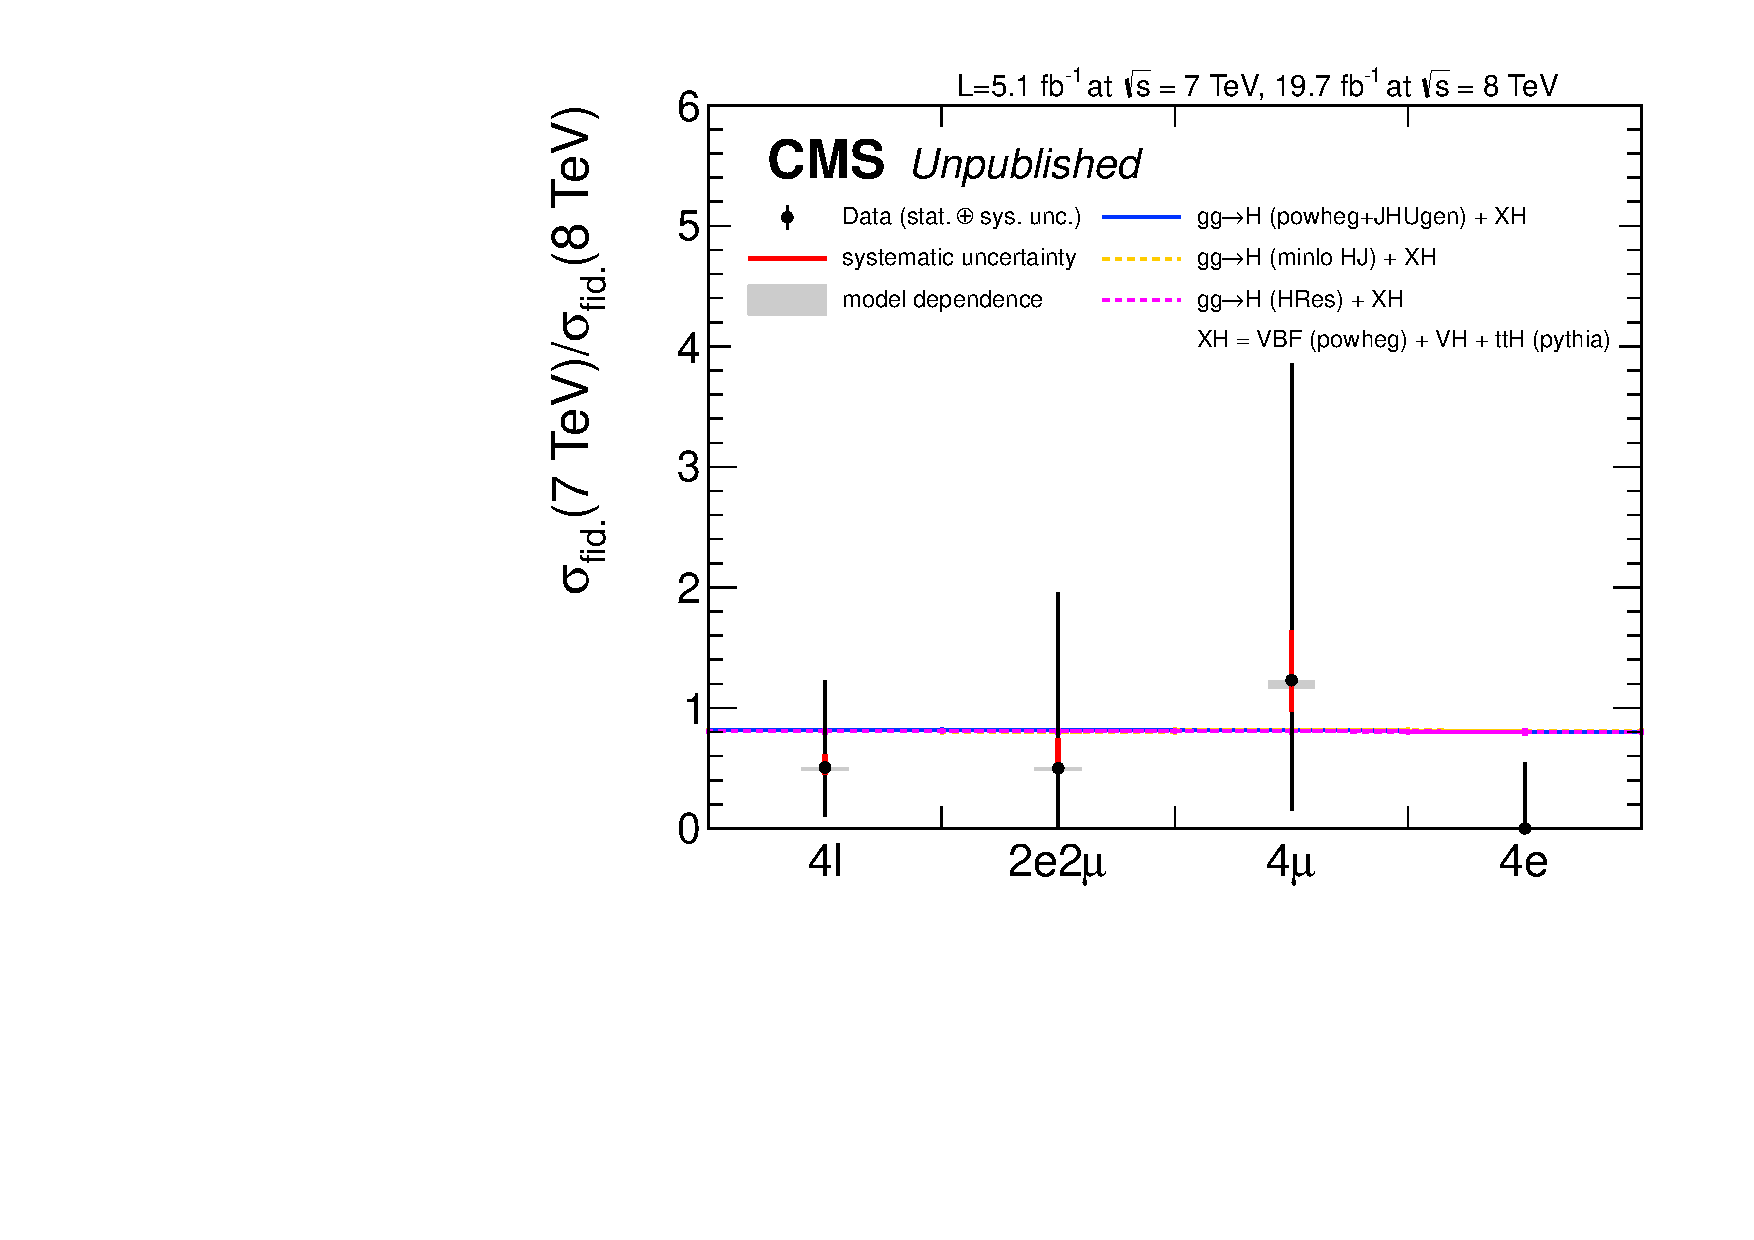
\includegraphics[width=0.65\textwidth,angle=0]{Plots/ratio7to8_mass4l_unfoldwith_SM_125_unpublished.pdf}
%    \caption{Ratio of fiducial cross sections of H$\rightarrow 4l$ at 7 and 8~TeV, and compassion to the theoretical estimates.
%     The SM NNLL+NNLO theoretical estimations where the shape of the dominant gg$\rightarrow$H contribution is modelled by {\sc HRes}, {\sc powheg+JHUgen} and
%     {\sc powheg minlo-HJJ}
%%     {\sc powheg minlo-HJ}
%      are shown in pink, blue and yellow, respectively. The red error bar represents the systematic uncertainty, while black error bar represents the combined statistical and systematic uncertainties, summed in quadrature. The additional systematic uncertainty associated with the model dependence is separately represented by a grey box.
% }
% \label{fig:ratio7o8-results-summary}
% \end{center}
%\end{figure}

%==================
 
The measurement of the integrated $\Hllll$ fiducial cross section using 13~TeV data is found to be nice agreement with the theoretical predictions 
within the corresponding uncertainties. The dominant and sub-dominant uncertainties on the measurement are systematic and statistical uncertainties which are about 24\% and  23\% respectively. The theoretical uncertainty is about FIXME: 11\%. 
 
%============
\begin{table}[!h!tb]
\begin{center}
      \caption{ 
The results of the $\Hllll$ integrated fiducial cross section measurement performed in the $m_{4\ell}$ range from 105~GeV to 140~GeV.
%	, and results of the $\Zllll$ integrated fiducial cross section measurement performed in the $m_{4\ell}$ range from 50~GeV to 105~GeV.
        } \label{tab:incresultsPAS}
\begin{tabular}{|c|c|c|c|c|}
\hline %---------------------------------------------------------
\hline %---------------------------------------------------------
\multicolumn{5}{|l|}{ Fiducial cross section H$\rightarrow 4l$ (fb) at 13~TeV. } \\
\hline %---------------------------------------------------------
& 4l & $2e2\mu$ & $4\mu$ & $4e$ \\
\hline %---------------------------------------------------------
\vspace{-0.4cm} &&&&\\
Measured (stat.~$\oplus$~sys.)(model)
&$1.11^{+0.43}_{-0.36}{}^{+0.08}_{-0.02}$
&$0.48^{+0.27}_{-0.22}{}^{+0.03}_{-0.03}$
&$0.26^{+0.17}_{-0.13}{}^{+0.01}_{-0.01}$
&$0.37^{+0.30}_{-0.22}{}^{+0.04}_{-0.02}$

\\
\vspace{-0.4cm} &&&&\\
\hline %---------------------------------------------------------
\vspace{-0.4cm} &&&&\\
\small gg$\rightarrow$H({\sc pohwheg}) + XH
&$1.16^{+0.11}_{-0.11}$
&$0.54^{+0.05}_{-0.05}$
&$0.33^{+0.03}_{-0.03}$
&$0.30^{+0.03}_{-0.03}$
\\
\vspace{-0.4cm} &&&&\\
\hline %---------------------------------------------------------
\vspace{-0.4cm} &&&&\\
%\small gg$\rightarrow$H({\sc minloHJJ}) + XH
\small gg$\rightarrow$H({\sc NNLOPS}) + XH
&$1.17^{+0.11}_{-0.11}$
&$0.54^{+0.05}_{-0.05}$
&$0.32^{+0.03}_{-0.03}$
&$0.29^{+0.03}_{-0.03}$
\\
\hline %---------------------------------------------------------
\hline %---------------------------------------------------------
%\multicolumn{5}{|l|}{ Fiducial cross section H$\rightarrow 4l$ (fb) at 7~TeV.} \\
%\hline %---------------------------------------------------------
%& 4l & $2e2\mu$ & $4\mu$ & $4e$ \\
%\hline %---------------------------------------------------------
%\vspace{-0.4cm} &&&&\\
%% Measured (stat.)(sys.)(model)
%Measured (stat.~$\oplus$~sys.)(model)
% & $0.56 {}^{+0.69}_{-0.44} {}^{+0.02}_{-0.02} $
% & $0.23 {}^{+0.58}_{-0.23} {}^{+0.01}_{-0.02} $
% & $0.32 {}^{+0.44}_{-0.27} {}^{+0.01}_{-0.01} $
% & $0.00 {}^{+0.17}_{-0.00} {}^{+0.00}_{-0.00} $
%
%\\
%\vspace{-0.4cm} &&&&\\
%\hline %---------------------------------------------------------
%\vspace{-0.4cm} &&&&\\
%\small gg$\rightarrow$H({\sc HRes}) + XH
%& $0.93^{+0.10}_{-0.11}$  & $0.44^{+0.05}_{-0.05}$  & $0.25^{+0.03}_{-0.03}$  & $0.24^{+0.03}_{-0.03}$  
%
%\vspace{-0.4cm} &&&&\\
%\hline %---------------------------------------------------------
%\vspace{-0.4cm} &&&&\\
%\small gg$\rightarrow$H({\sc pohwheg+JHUgen}) + XH
%& $0.94^{+0.10}_{-0.10}$  & $0.44^{+0.05}_{-0.05}$  & $0.27^{+0.03}_{-0.03}$  & $0.24^{+0.03}_{-0.03}$ \\
%\vspace{-0.4cm} &&&&\\
%\hline %---------------------------------------------------------
%\vspace{-0.4cm} &&&&\\
%%\small gg$\rightarrow$H({\sc minloHJJ}) + XH
%\small gg$\rightarrow$H({\sc minloHJ}) + XH
%& $0.93^{+0.10}_{-0.10}$  & $0.43^{+0.05}_{-0.05}$  & $0.26^{+0.03}_{-0.03}$  & $0.23^{+0.02}_{-0.02}$  \\
%\hline %---------------------------------------------------------
%\hline %---------------------------------------------------------
\end{tabular}
\end{center}
\end{table}
%============
